% leastUPO.tex
%
% Predrag created file              Apr 12 2007
% $Author$ $Date$


\subsection{Least unstable \rpo s ???}

\PC{serious work/pruning needed here}
Hence plot all \rpo s in these 2 representations:

$[ \Re a_2, \Im a_2, \Re a_3 ]$
(here 2-\eqv\  is a circle, 3-\eqv\ a vertical line)
 and
$[ \Re a_3, \Im a_3, \Re a_2 ]$
(here 3-\eqv\ is a circle, 2-\eqv\ a vertical line)

\ES{
The names of the \rpo\ figure files follow the convention
 {\tt rpoL-T-d.eps}s, with suffixes {\tt cm}
and {\tt u} indicating
 mean velocity frame  and $u$ representation respectively.
   }
%
Out of 30 \rpo s we
find,  only three are truly periodic.  The orbit
with $\period{p} = 95.25$ has a very small
$d = -6.5\,\times 10^{-7}$, but it is not periodic
(we
checked this by decreasing the integration step size and increasing the
number of modes).


%%%%%%%%%%%%%%%%%%%%%%%%%%%%%%%%%%%%%%%%%%%%%%%%%%%%%%%%%%%%%%%%
\begin{figure}[t] \label{f:rpo55}
\begin{center}
(a) 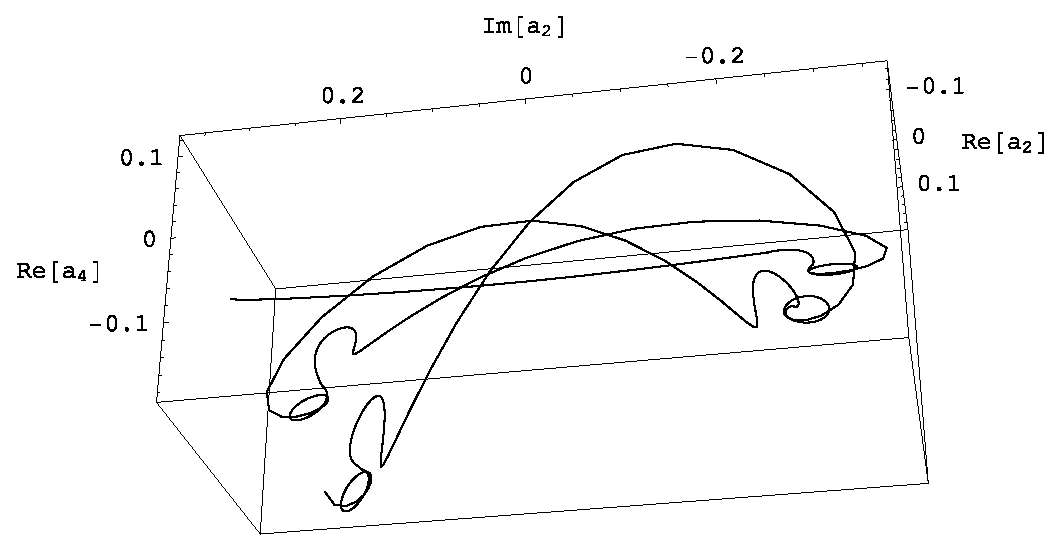
\includegraphics[width=0.35\textwidth]{figs/rpo22-55-4-clean.eps}
% ./removecache.sh rpo22-55-4.eps
% abandoned rpoEq22-55-4.eps with mean velocity equilibrium embeded.
(b) 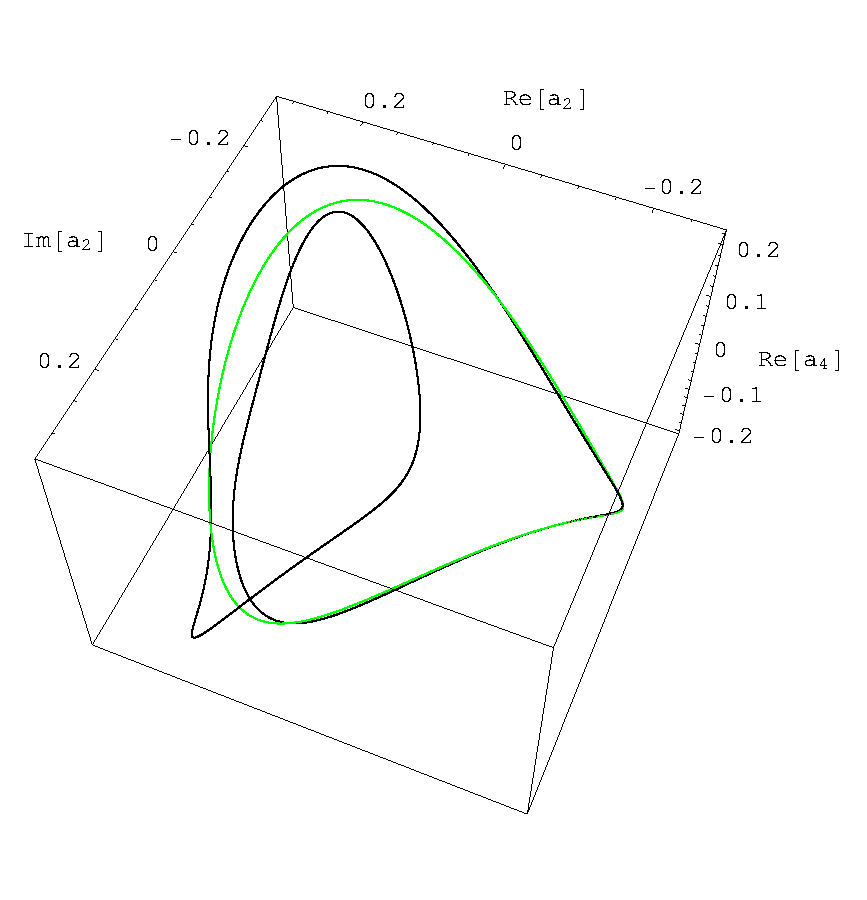
\includegraphics[width=0.25\textwidth]{figs/rpoEq22-55-4-cm.eps}
(c) [create rpoEq22-55-4-cm-?.eps]
\end{center}
\caption{
 The \rpo\ {\nameit}55 in:
 (a) \Statesp, traced for four periods $\period{p}$.
% Green curve belongs to \reffig{f:rpo55}(b) % rpo22-55-4-cm.eps
% rather than to  \reffig{f:rpo55}(a), % rpoEq22-55-4.eps?
 (b) mean velocity frame.
        The continuos family of
    {\eqva} A obtained by the action of $g$ is shown in green,
    the SA family shown in red. The \rpo\ {\nameit}55 stays close
    to either A or SA for close to 1/2 of {\eqv} rotation
    period, then quickly jumps to the other {\eqv} point.
 (c) mean velocity frame A, SA and {\nameit}55 projected on the
    $[a_?,a_?]$ plane,
    with the $\sigma x = -x$ symmetry of \KSe\ explicit.
        }
\end{figure}
%%%%%%%%%%%%%%%%%%%%%%%%%%%%%%%%%%%%%%%%%%%%%%%%%%%%%%%%%%%%%%%%%%



Sets of \rpo s are difficult to visualize simultaneously.
For ordinary \po s one
plots the unstable plane of the \eqv, shows where the periodic
orbits sit. Other options:

Somewhat better visualization is in the
{\em mean velocity frame}, {\ie}
a reference frame that rotates with with velocity
$v_p=\shift_p/\period{p}$
In the mean velocity frame a \rpo\ becomes
a \po, see  for example \refeq{f:rpo55}.
Mean velocity frame visualization helps quite a bit.
Put a black (green, respectively) dot
twice thickness of the line every time unit; it will enable you to see
where the motion is slow and where it is fast.
% (a trick we used to understand plane Couette trajectories).
Mark the initial point on both
mean velocity \rpo\ and on \eqv\  in mean velocity
 frame with a fat triangle
indicating the direction, so we can see how they both move. Probably at the
opposite ends of the two curves - mean velocity frame is the mean motion.

%   rpo/figs/detail1rpo22-55-4.eps
%   rpo/figs/detail2rpo22-55-4.eps
%   rpo/figs/detail3rpo22-55-4.eps
%   break rpo22-55-4 into 3 parts.
%   The script for the fonts somehow crops these images

Each {\rpo} has its own mean velocity frame - and within it, {\eqv}
move on circles (or worse - because in higher Fourier modes they do more
complicated things), and it is important to know where the {\eqv} is at
a given instant.

As the shift $d$ is defined mod~$L$, better to
state for each {\rpo} its mean velocity $c_p = \shift_p/\period{p}$,
where $\shift_p$ is measured on the line (not on the circle). $c_p$ is
preferable to angle $2\pi \shift_p/L$ as it does not vary in $L \to$~large
limit (just like $\sqrt{2}$ wavelength estimate is independent of
system size).

Another convenient way to plot \eqva\ and \reqva\ on a periodic
domain $L$ is to plot
$\partial u(x)$ vs. $u(x)$ as a curve parametrized by
$x\in [0,L]$. In this representation both \eqva\ and \reqva\ curves are
stationary, but the points on \reqva\ move as functions of time.

\Po s and \rpo s can be plotted this way as well
$u_x(x,t)$ vs. $u(x,t)$. Now they are are represented by time-dependent
``tube".

\refFig{f:ks22RE}(b)
depicts \REQV{+}{2}.
It belongs to the branch starting at point $M$
\PC{does it start at M?}
in bifurcation diagram \reffig{fig:ksBifDiag}.
It has one real unstable eigenvalue = 0.337,
so it is more unstable than \REQV{+}{1},
but only in 1\dmn\ (\REQV{+}{1} is unstable in 4\dmn).
\PC{removed Ruslan Feb 8 2007 Fig f:TW1TW2.ps in favor of fresher version}
